\chapter[Computer vision and CNN]{Computer vision and Convolutional Neural Networks}

\textbf{Computer Vision} is a field of Artificial Intelligence which aims to implement models that performs visual tasks. Some of the tasks in this field are for example: \textit{image classification}, \textit{object detection} within an image, the so-called \textit{neural style transfer} and so on. All of this tasks, for the nature of input data, involves an enormous number of features which corresponds to a huge number of parameters to learn. How we have said several times, a \textit{classical neural network} (shallow) for example, cannot perform properly and in acceptable time such a task. Just for give an idea, the number of parameters to lean can be also around a billion! For this reason \textbf{convolutional architectures}, and then \textbf{convolutional neural networks} are introduced.

\section{Convolutional Neural Networks: main ingredients}
A \textbf{Convolutional  Neural Network} (\textbf{CNN}) is made up of several parts: (i) a \textit{convolutional layer}, (ii) a \textit{pooling layer}, (iii) a \textit{fully connected layer}.

\subsection{Convolution}
This is the core building block of a CNN, here the great majority of the computation occurs; there are several levels of this type. Besides, the convolutional layers are the ones in which the network learns the main feature from the input data. In the case of images, passing through the convolutional part of the NN low level to high level features are learned. The following figure shows an example of the extracted details at different levels of the architecture:

\begin{figure}[h]
    \centering
    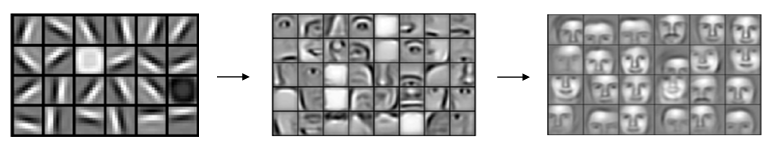
\includegraphics[scale=0.8]{img/CNN_example.png} 
\end{figure}

\noindent
You can see in the first stage only some edges are detected, passing through more complicate details arriving to the detection of entire faces. \\
This procedure takes inspiration on how our brain solve the problems; biological studies have confirmed that in order to perform a certain task, our brain solves, step by step, simpler problems in order to reach more complicate ones.\\
From now on, we are going to focus our attention on \textbf{images}, and in particular we are going deeper in some details on \textit{how convolution process works}.\\

The \textit{convolution} requires few components: (a) input data, (b) a \textbf{filter}, (c) a \textbf{feature map}. Considering that an image can be seen as a matrix of pixels, roughly speaking the filter moves across the image checking if the feature for which that filter itself has been built, is present. This process is known as \textbf{convolution}.

In the following there is a figure that shows, mathematically speaking, what are the main steps behind such a procedure.

\begin{figure}[h]
    \centering
    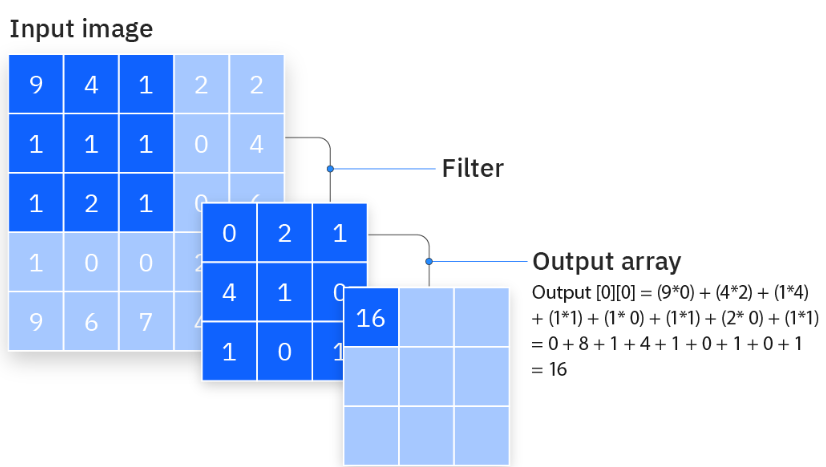
\includegraphics[scale=0.8]{img/convolution.png}
    \caption{Convolution: main steps}
\end{figure}

\noindent
In practical terms also a filter is a square matrix (with \textit{odd dimension}) in a way that it has a center. Such a filter is \textit{convolved} to the image in the sense it slides across subregions of it which have the same dimension of the feature detector; the output array (another matrix called the \textbf{feature map}) is done by scalars corresponding to the sum of the product element by element of the involved matrices. \\
How we will see, part of the parameters that the the network has to learn are those constituting such filters, then no one tells to the network how to find edges (also at different inclination) or other types of details!\\
 It should be clear that, going across the process of convolution the dimension of the matrices is reduced. In particular: starting from an image (square for simplicity) $n\times{n}$, by applying on it a filter $f\times{f}$ the dimension of the ouput will be shrinked by a quantity $f-1$ (for each dimension), with a resulting size of $(n-f+1)\times{(n-f+1)}$.

\subsubsection{Padding}
We can add a frame of padding to the image (usually by adding zeros) in order to avoid the phenomenon of \textit{shrinking dimensions}. Then, if a padding of $p$ is added to the input image (so that it results in being $(n+p)\times(n+p)$) and an $f\times{f}$ filter is applied the resulting image will have shape $(n+2p-f+1)\times{(n+2p-f+1)}$.

%%TODO: Uso il padding anche perché altrimenti perderei delle informazioni ai bordi dell'immagine

\begin{figure}
    \centering
    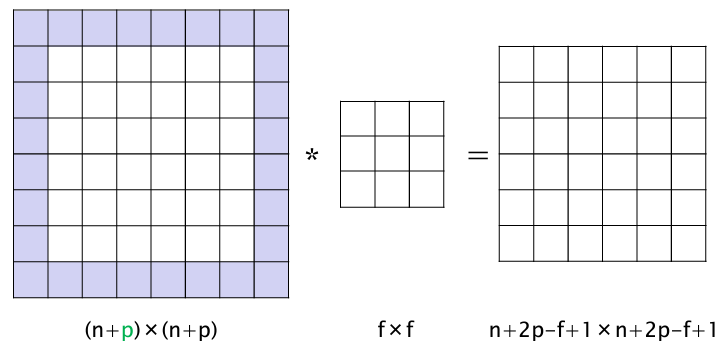
\includegraphics[scale=0.6]{img/CNN_padding.png}
    \caption{Image padding for avoiding dimension reduction}
\end{figure}

Only for a matter of nomenclature, we have to say that a convolution which does not use the padding is called \textit{valid convolution}, otherwise we have a \textit{same convolution}. The \textbf{amount of padding} to be added is such that the input and ouput images have exactly the same shape. By doing simple calculations we can find that this quantity is equal to $p=(f-1)/2$, it gives always a non-fractional value since $f$ is known to be odd.

%Attenzione qua: s=1 vuol dire nessun pixel saltato (mi sposto di uno ogni volta cioè non salto nulla)
\subsubsection{Strided convolutions}
The last step is needed to complete the overview on the first part of CNN: \textbf{strided convolutions}. Whether in the procedure of applying the kernel some pixels (cells of the matrix) are skipped, then the procedure is known to be \textbf{strided}. A number of skipped cells greater than one is rare, however it is remarkable that also in this case the dimension of the feature map is shrinked. More clearly, for a stride $s$ the dimensions for the output are: 
\begin{equation*}
    \left\lfloor \frac{n+2p-f}{s}+1\right\rfloor\times
    \left\lfloor \frac{n+2p-f}{s}+1\right\rfloor
\end{equation*}
How you will imagine, after some chapter of discussion on NN, such an $s$ is another hyperparameter (usually $s=1$, if a \textit{same convolution}) is used.

%TODO: Quando le dimensioni non sono sufficienti certe combinazioni vengono saltate (per convenzione). Qui l'obiettivo è quello di ridurre la dimensione dell'output al contrario del padding.

% Convoluzione --> combinazione lineare
% Padding --> Mantenere dimensione output
% Strided convolution --> Ridurre output

\subsection{Convolutions on RGB images}
In the previous paragraphs, for sake of clarity about the main aspects of convolution, we have implied that the image for which we were training the CNN was a gray-scale one. A part from few tasks, nowadays colored images are used.
Let us suppose, without loss of generality, on the contrary they are RGB ones. This implies that now the input images are not 2D-arrays anymore, they are 3D since there is an $n\times{n}$ matrix for each one of the three channels R, G, B. A \textit{3D-kernel} is needed as the number of channels. Despite the shape of the inputs is changed, what is not changing is the simple computational procedure, since all of the values are summed up! Then the feature map is always a 2D-array and the network is clearly allowed to use different or same filters. 

\subsubsection{Multiple Filters}
In the case that at this stage \textit{multiple filters} are used, also the output has a three-dimensional shape.
Now, whether on a RGB image whose shape is ${n}\times{n}\times{n_C}$, is applied $n_C'$ (number of channels of the output) filters whose shape is ${f}\times{f}\times{n_C}$ (with $n_C$ being the number of channels) $\to$ the output shape will be (no padding, no striding) $(n-f+1)\times(n-f+1)\times{n_C'}$.\\

\begin{figure}[h]
    \centering
    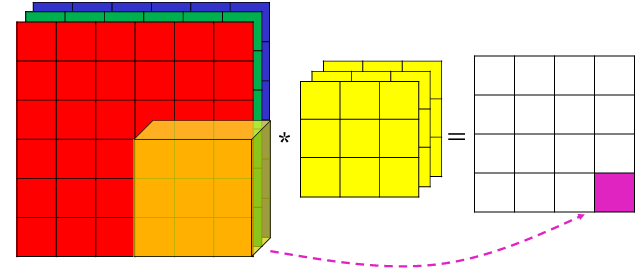
\includegraphics[scale=0.6]{img/CNN_RGB.png}
    \caption{Convolution on RGB images producing 2D-output}
\end{figure}

We can see that the convolution operation is nothing but a (just more complicated) linear combination. This is the counterpart of $z$ in the linear regression, then -- also here -- a \textit{nonlinear part} is missing! In fact, before passing the output to the next layer, even in this case an activation function is employed, in particular the ReLU. This prepares the activations for the next layer. Such a situation is well depicted in the following:

\begin{figure}[h]
    \centering
    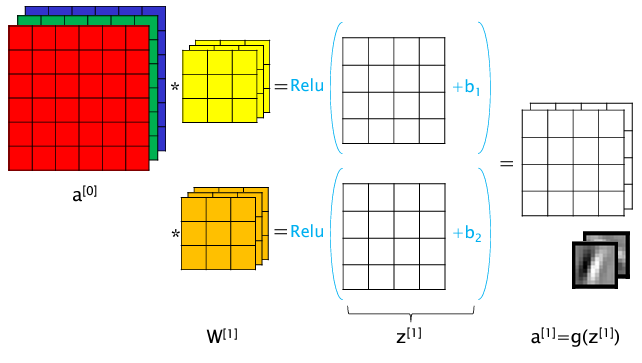
\includegraphics[scale=0.7]{img/ReLU_CNN.png}
    \caption{ReLU on feature maps}
\end{figure}

\subsubsection{Example: Number of parameters in a CNN}
How many parameters we have in a layer of a convolutional neural network which use \textit{10 filters} $3\times3\times3$? For a single filter we have:  $3\times3$ parameter for each 'sheet', there are 3 sheets for a filter, then for a single filter we have 27 parameters. Furthermore, there is another parameter for each filter which is related to the bias which is added before passing for the ReLU. Since we have 10 filters, the total number of parameters is 
\begin{equation*}
    (3\times3+1)\times10=280
\end{equation*}

\subsection{Notation}
Here we introduce some notation which will be useful in the comprehension of the examples of CNNs. Suppose we have the $\ell$-th convolutional layer, for such a layer we can have some filters of dimension $f^{[l]}$ (they are square), we could apply some padding and/or stride, respectively $p^{[l]}$ and $s^{[l]}$. Then, the \textbf{input} will have dimension $n_H^{[l-1]}\times{n_W^{[l-1]}}\times{n_C^{[l-1]}}$, while \textbf{the output} will have dimension $n_H^{[l]}\times{n_W^{[l]}}\times{n_C^{[l]}}$, where $n_C^{[l]}$ is the number of filters for the $\ell$-th layer, while $n_{H/W}^{[l]}$ is equal to:
\begin{equation}
    \left\lfloor \frac{n^{[l-1]}+2p^{[l]}-f^{[l]}}{s^{[l]}}+1\right\rfloor
\end{equation}
\textbf{Each filter} has dimension $f^{[l]}\times{f^{[l]}}\times{n_c^{[l]}}$, the dimension for an activation for a certain layer is equal to the output, since we have $m$ examples we have $m$ times the dimension of the output. All of the activations are indicated with $A^{[l-1]}$. The \textbf{number of parameters} for a layer is:
\begin{equation}
    f^{[l]}\times{f^{[l]}}\times{n_C^{[l-1]}}\times{n_C^{[l]}}+n_C^{[l]}
\end{equation}
Note here that a filter has a dimension that is equal to the dimension of the output of the previous layer.
In the following an example is showed in which there are 4 convolutional layers:

\begin{figure}[h]
    \centering
    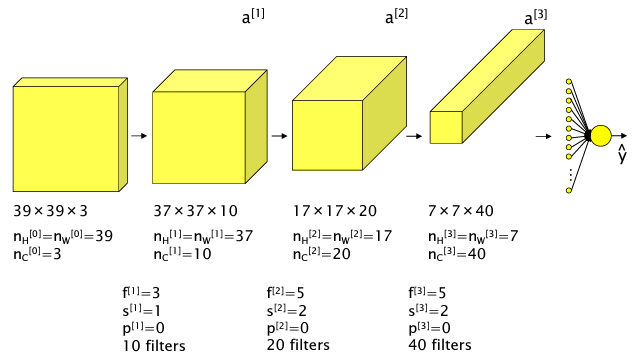
\includegraphics[scale=0.8]{img/ConvNet_Example.png}
    \caption{Example of a CNN (with all the dimensions)}
\end{figure}


\subsection{Pooling layer: Max-Pooling}
Once also the ReLU has been computed, the output is further modified. A \textbf{pooling function} replaces the output of the net for a certain location with a \textit{summary statistic} of the nearby outputs. The most commons are the \textbf{max-pooling} and the \textbf{average-pooling}. The type of statistic to be used is a user-defined choice. The introduction of pooling bring with itself other two hyperparameters, the dimension of the \textit{neighbourhood} on which the pooling is applied, the stride by which this occurs.

\begin{figure}[h] \label{fig: CNN_example}
    \centering
    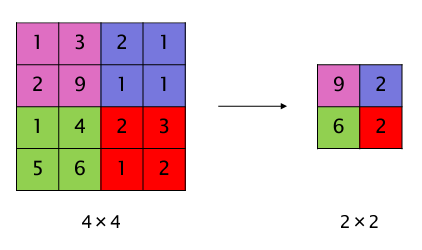
\includegraphics[scale=0.7]{img/MaxPooling.png}
\end{figure}

In this case the added hyperparameters are $f=2$ (dimension of the sub-blocks) and $s=2$ since at each pooling stage a cell is skipped. \\
Clearly the pooling reduces the dimension of the activations, but it is useful in order to summarize the information obtained at a certain stage. It is remarkable that different than the convolution stage, the pooling stage is performed separately for each channel of given activations.

\subsection{Fully connected layer}
The convolutional layers -- made up of convolutional and pooling stage -- works as feature extractors, finally at the end of the architecture some \textit{fully connected layers} are present, they carries out the work of classifying a given example, then the last layer is a \textit{softmax} one, which gives for each class a probability for the sample to be part of a certain class. 
Look at the Figure (\ref{fig: CNN_example}), for the last  volume if we isolate a single cell, this is nothing but a linear combination of the parameters plus a bias, this is a neuron! Then the first fully connected (Dense) layer is nothing but the unrolling of all of the neurons contained in the last volume.\\

\noindent
As first example, the CNN for the \textit{digit classification is given} (see \cite{lenet5} for further information):

\begin{figure}
    \centering
    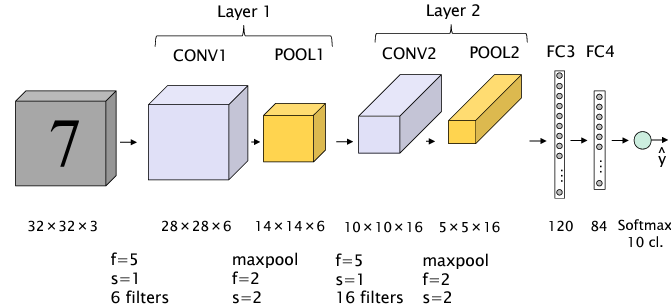
\includegraphics[scale=0.7]{img/LeNet_digit.png}
    \caption{\textbf{LeNet-5}: CNN for digit recognition}
\end{figure}
Note how the pooling stage does not change the third dimension (the depth of the volume) but only the height and width. As usual the last volume from POOL2 is unrolled in some computational units which made up the first layer for the fully connected part of the network. \\
In the pooling stage there are no learned parameters since only a statistic summary is done on subregion of the activations.

\subsection{Why Convolutions?}
The convolutional stage is very used, mainly for two aspects: 
\begin{itemize}
    \itemsep-0.3em 
    \item \textbf{Parameter sharing}: when a filter for a part of the image is used (eg. edge detection) probably it will be useful also for another part of the image; the same parameters used for different part of an image and (why not) for other images in which the same low/high level features, could be detected.
    \item \textbf{Sparsity of connections}: at each layer the outputs depend on a small number of inputs.
\end{itemize}
It could appear strange, but in a CNN the great majority of the parameters are concentrated in the fully connected layers! This is one of the reason why shallow fully connected networks performs very bad in terms of image classification.

\section{Case studies and tasks}
In the following some examples of CNN architectures are reported, for sake of completeness also the paper are cited.

\subsection{AlexNet}
This type of architecture was introduced in \cite{AlexNet}, and the objective was the image classification, differently from \textit{LeNet-5} having 2 convolutional layers, this architecture contains 6 convolutional layers. The depth of the network was relevant for the obtained results which opened the road to a lot of studies on computer vision. The AlexNet paper is one of the most cited ones especially for the obtained results. Just for give an idea, the training set had 1.2 million images. It was trained for 90 epochs, which took five to six days on two NVIDIA GTX 580 3GB GPUs which had been working in parallel. 

\begin{figure}[h]
    \centering
    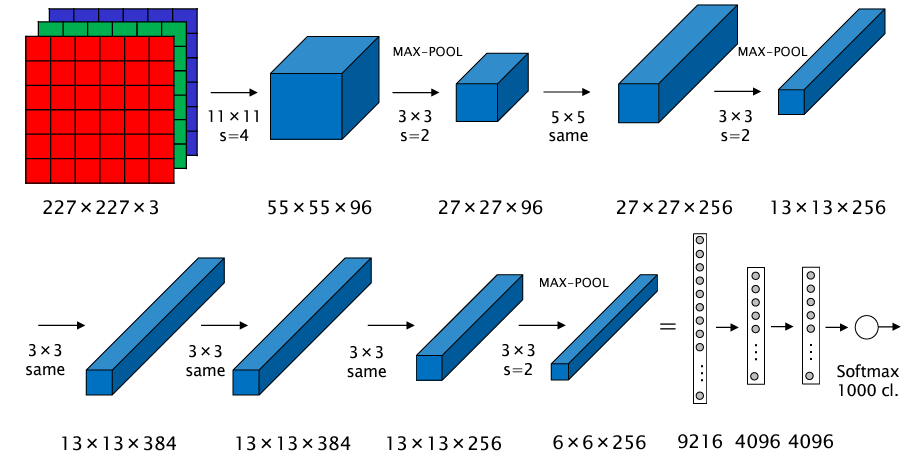
\includegraphics[scale=0.6]{img/AlexNet.png}
    \caption{\textbf{AlexNet} architecture}
\end{figure}

\subsection{VGG-16}
They are named after the \textit{Visual Geometry Group (VGG)} of the Oxford University. The full description of the net can be found in \cite{VGG-16}. 16 is the number of its layers (13 convolutional, 3 deep), there are other VGG networks with a different number of layers.

\begin{figure}[h]
    \centering 
    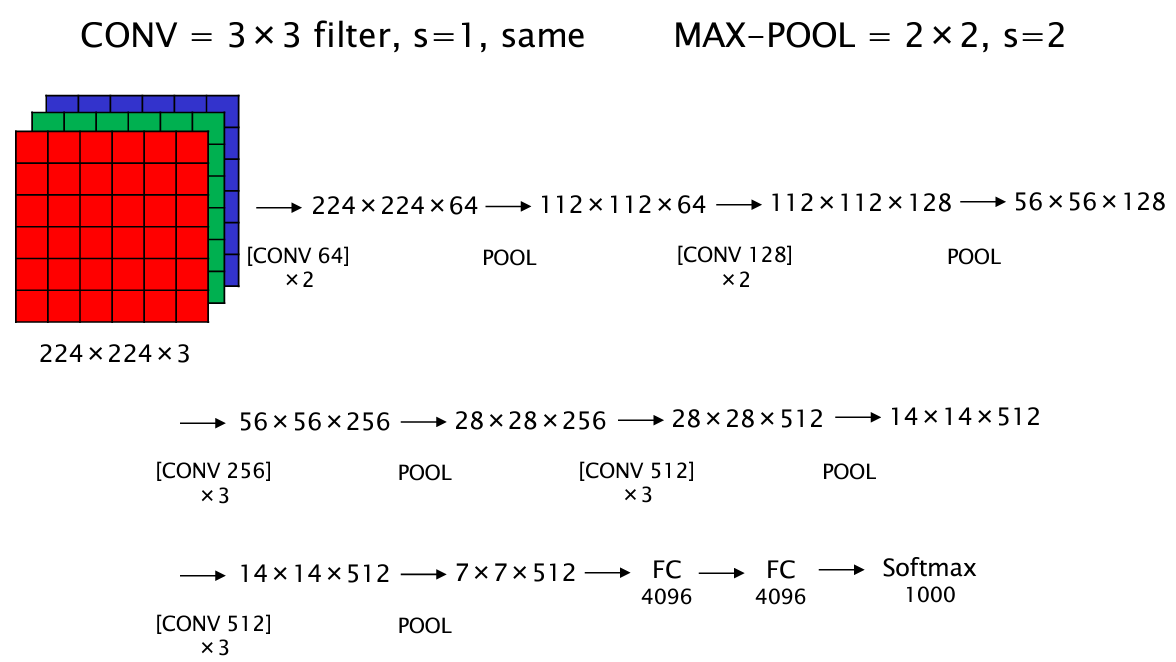
\includegraphics[scale=0.5]{img/VGG16.png}
    \caption{\textbf{VGG-16} architecture}
\end{figure}

\subsection{Residual Network(ResNet)}
Till now we have mentioned the structures of the DNN \textit{LeNet, AlexNet, VGG-16}. In a similar way we could build up our deep neural network, ma in the practice they are hard to train. Residual Networks allow us to perform a more efficient training of them. \\
We have seen in the previous paragraph that DNNs suffer the problem of the \textit{vanishing gradient}, we can say that data is disappearing through the network. Some reaserchers from Microsoft found that the split of a deep network into chuncks help eliminate much of this disappearing signal problem. In other words \textit{ResNets} breaks down  a very deep plain neural network into \textbf{small chuncks of network} connected each other by using \textit{skip} or \textit{shortcut connections}.


\begin{figure}[h]
    \centering
    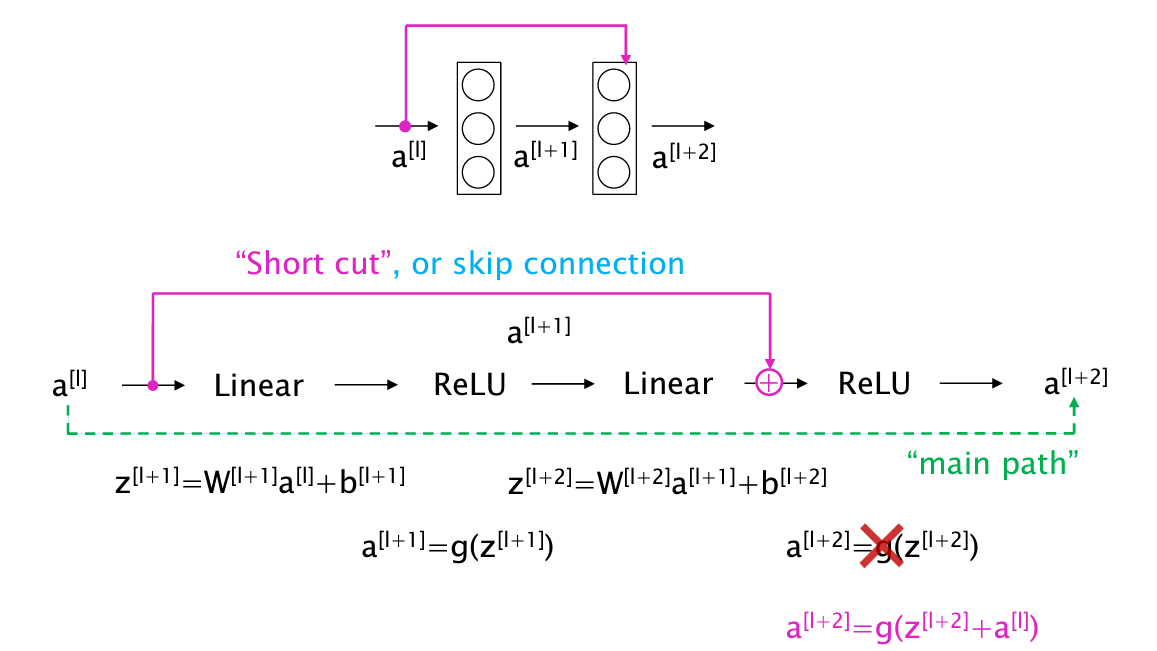
\includegraphics[scale=0.5]{img/ResNet.png}
    \caption{\textbf{ResNet} skip connections}
\end{figure}
\noindent
In the figure above we can see the core constituting ResNets: \textbf{skip connections}. Roughly speaking the activation of the layer $l+2$ are computed using also the activation from the layer $l$. In this sense there is a skip through the layers. On such a type of architecture we have that the training error curve is how we can expect from the theory, differently from the \textit{plain neural networks}. In the following we show an example of ResNet with 34 layers in which \textit{skip connections} are used. The number of layers skipped is two, but "very surprisingly" the number of skipped layers can become another hyperparameter. In the original case presented in \cite{ResNet} the skip connection is from the level $l\to{l+2}$, that is the activation of the level $l$ influences the ones in the level $l+2$.

\begin{figure}[h]
    \centering 
    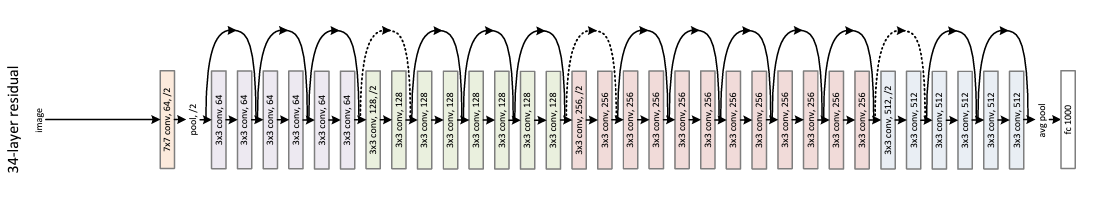
\includegraphics[scale=0.6]{img/ResNet2.png}
    \caption{Example of 34-layers ResNet}
\end{figure}

\section{${1}\times{1}$ convolutions}
We have seen that in the convolutional stage some filters are applied in order to produce a linear combination of the input data. Could be strange, but there are some cases in which doing a $1\times{1}$ convolution is useful in order to reduce the number of computations, since the number of multiplications is directly proportional to the dimension of the filter! \\
Now, suppose we have an initial volume as the one represented in blue and we apply a filter as the one in yellow, we are doing nothing but the computation that occurs in a neuron (a part from the ReLU which is performed at the end): the $1{\times}{1}\times{32}$ filter applied to the volume gives us a linear combination of the input at the same Height and Width, but on different channels through the parameters contained into the filter. This is the reason why such a type of procedure is called \textit{Network-In-Network} (see \cite{NetInNet} for further details), this clearly reduces the number of multiplications that are performed.

\begin{figure}[h]
    \centering
    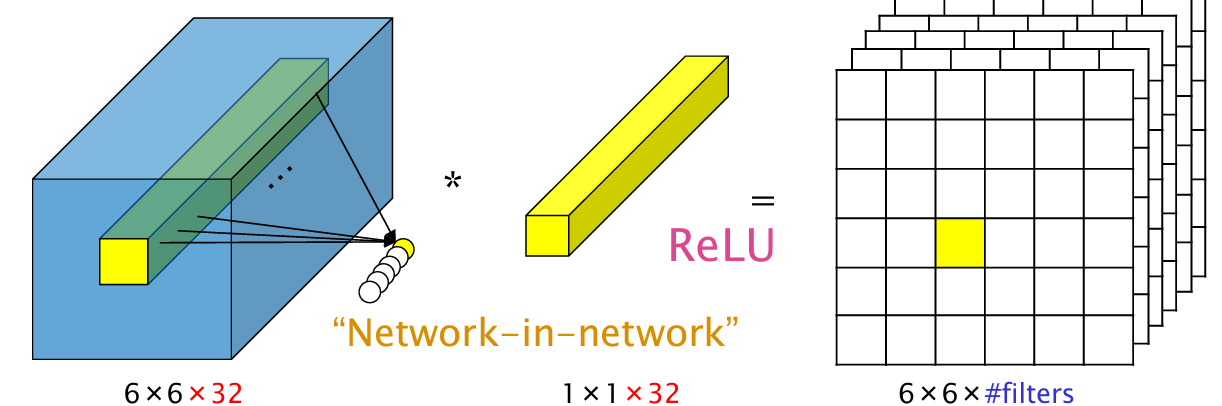
\includegraphics[scale=0.6]{img/NiN.png}
    \caption{Network-In-Network and $1{\times}{1}$ convolutions}
\end{figure}


\subsection{Inception: another DNN architecture}
From the ideas presented in \cite{NetInNet} and with the increasing in computation capabilities, in Google was created a new CNN architecture who has been called \textbf{Inception} (see \cite{Inception}) (from a famous film from which they was inspired, in particular by an iconic phrase appeared in a meme \textit{"We need to go deeper"}). Such a network has 22 layers, the great majority of them are inception modules, which are a culmination of the results presented in \cite{NetInNet}. Such an CNN is one the most used  architecture in computer vision.

\begin{figure}[h]
    \centering
    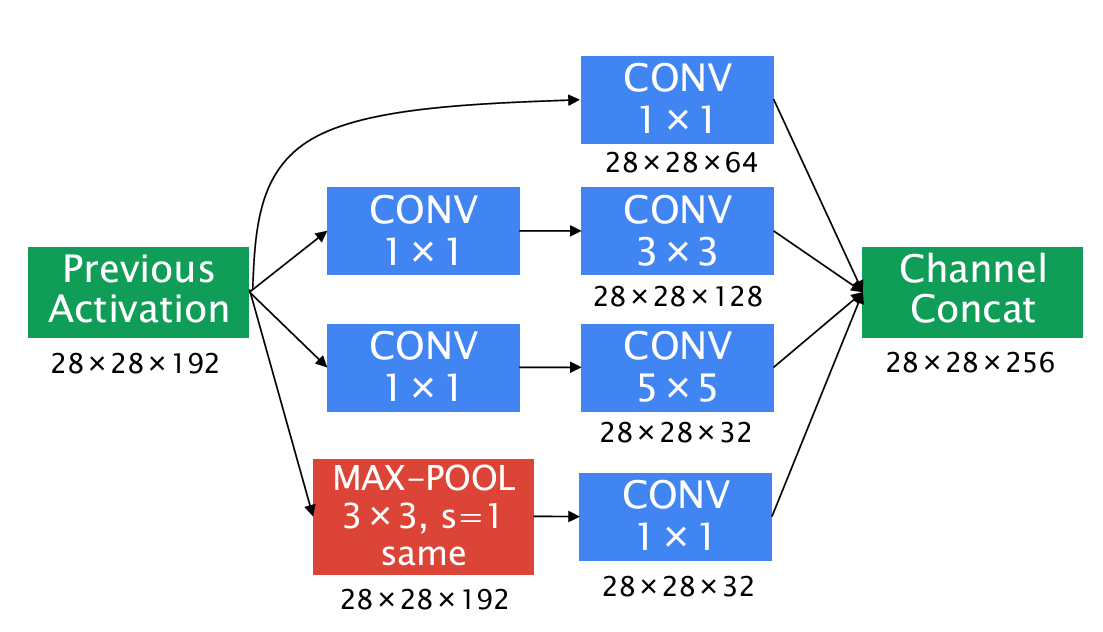
\includegraphics[scale=0.3]{img/InceptionModule.png}
    \caption{An Inception Module}
\end{figure}

\noindent
In an \textit{inception module} some $1{\times}{1}$ convolutions are used in order to reduce the number of computations of a 10 factor.
The main motivation behind the Inception modules is that DNN performs better if the number of layers is increased (that is the dimension of the network is increased).\\

\noindent
At the end of this discussion about DNN a graph in which the perfromances of the presented architectures is compared to the \textit{human/Bayes error}. 

\begin{figure}[h]
    \centering
    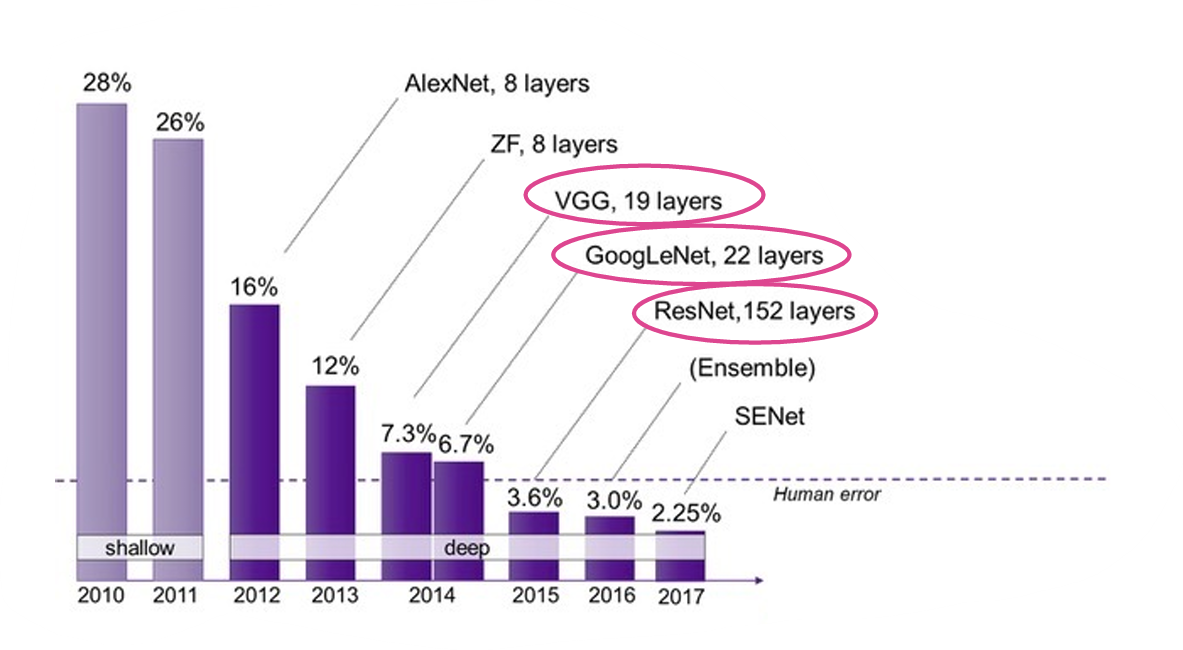
\includegraphics[scale=0.5]{img/PerfDNN.png}
    \caption{DNN performances vs human error}
\end{figure}

